\chapter{Base robotica Otto}

Otto è un robot a guida differenziale, progetto di ricerca del laboratorio di robotica IRALab, dell’Università degli Studi di Milano-Bicocca.

\section{Base robotica VolksBot RT 3}
VolksBot è un kit modulare per la costruzione di robot, progettato per il campo della ricerca e della  prototipazione rapida.
La base robotica è pensata per essere facilmente modificata ed adattata alle proprie esigenze in quanto composta da barre in alluminio combinabili fra di loro. \\
Nello specifico la base robotica utilizzata è composta da due ruote motrici frontali e una ruota basculante di supporto posteriore.
Ciascuna ruota motrice è collegata ad un motore a corrente continua combinato con una riduzione con un rapporto di trasmissione 1:74.
L'intero sistema robotico è alimentato tramite batterie a bordo del veicolo.
\begin{figure}[H]
\centering
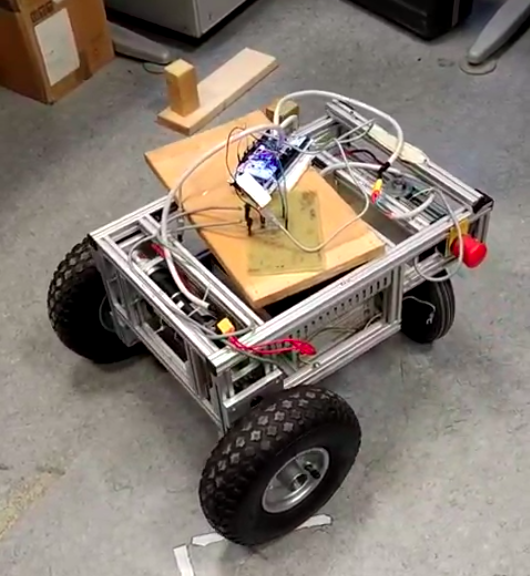
\includegraphics[scale=0.45]{images/otto1.png}
\caption{Base robotica Otto}
\end{figure}

\section{Encoder}
Un encoder è dispositivo elettromeccanico in grado di convertire la posizione o il moto angolare in un codice digitale.
Nel nostro caso è stato montato un encoder in quadratura sull'asse del motore di ciascuna ruota motrice.
Questo tipo di sensore è formato da un LED, da una corona circolare con un pattern fisso che si ripete e da dei fotodiodi. \\

\begin{figure}[H]
\centering
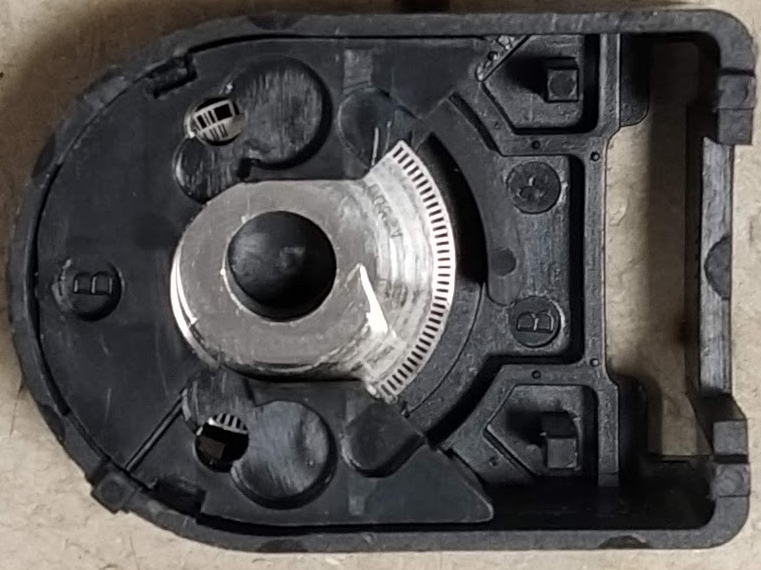
\includegraphics[scale=0.30]{images/corona.png}
\caption{Corona circolare dell'encoder}
\end{figure}

Il funzionamento si basa sulla capacità dei fotodiodi di percepire i cambiamenti di luce: il LED viene sempre alimentato ed emette quindi una luce costante, la corona dell'encoder gira insieme all'albero del motore e i fotodiodi rilevano i cambiamenti di luce dovuti al pattern sulla corona e tramite dei comparatori generano delle onde quadre.
Elaborando questi segnali è possibile misurare sia la distanza percorsa dalle ruote che la direzione del movimento.

\begin{figure}[H]
\hfill
\subfigure[Schema dell'encoder]{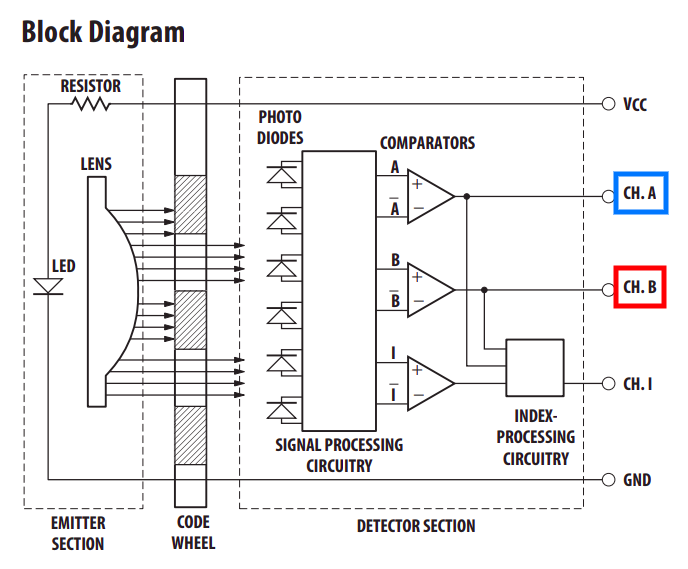
\includegraphics[scale=0.32]{images/encoder-1.png}}
\hfill
\subfigure[Segnale generato]{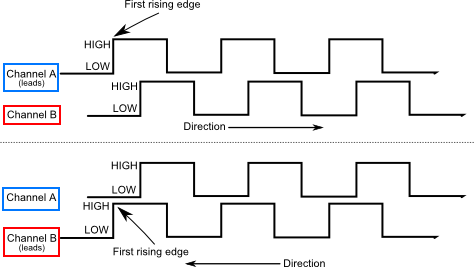
\includegraphics[scale=0.47]{images/quad-encoding-waveform-1.png}}
\hfill
\caption{Encoder in quadratura}
\end{figure}

\section{Motor driver}
Un motor driver è un dispositivo elettronico necessario per poter controllare i motori DC usando i segnali digitali generati da un microcontrollore.
Il circuito elettronico principale è chiamato ponte H e permette di controllare la polarità della tensione applicata a un carico. Tramite questo meccanismo siamo in grado sia di controllare la direzione del moto di un motore a corrente continua, stabilendo il verso nel quale fluisce la corrente, sia di regolare la velocità del motore modulando la tensione. \\
La modulazione della tensione avviene tramite un segnale PWM (pulse-width modulation). Questo segnale periodico ha due fasi: una in cui la tensione è alta (3.3V) e una fase in cui la tensione è bassa (0V). Il rapporto tra queste due fasi è detto duty-cycle e determina la tensione media in uscita.

\begin{figure}[H]
\centering
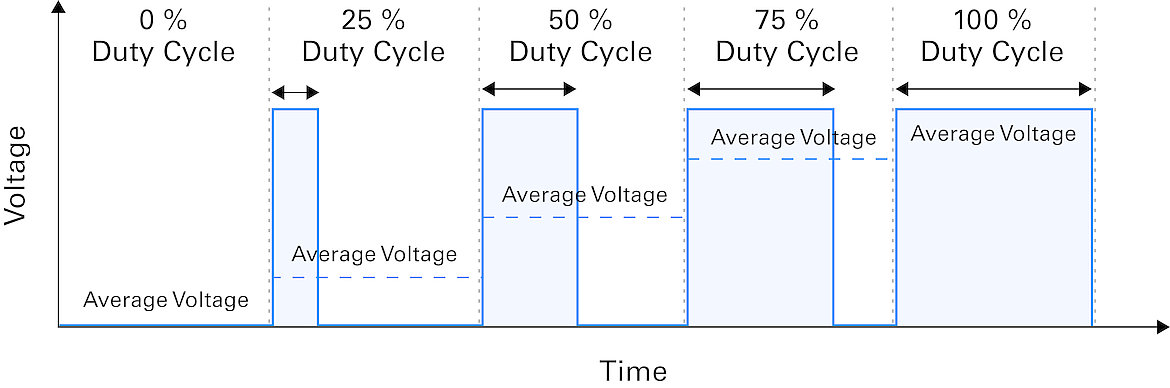
\includegraphics[scale=1.4]{images/pwm.jpg}
\caption{Modulazione della tensione con segnale PWM.}
\end{figure}


Il motor driver scelto è Pololu Dual G2: questo dispositivo ha due circuiti H-bridge, così da poter controllare entrambi i motori in modo indipendente.
Per controllare ciascun motore sono presenti 3 segnali di input:
\begin{itemize}
    \item SLP: disabilita l'output se è uguale a 0
    \item PWM: input particolare rappresentabile come percentuale, modula la velocità
    \item DIR: imposta la direzione di azione del motore
\end{itemize}

Si hanno quindi le seguenti modalità di funzionamento:
\begin{table}[H]
    \centering
    \begin{tabular}{|l|l|l|l|}
    \hline
    SLP & DIR & PWM & Operazione                            \\ \hline
    1   & 0   & \%pwm & motore azionato in senso orario a velocità pwm \\
    1   & 1   & \%pwm & motore azionato in senso antiorario a velocità pwm         \\
    1   & x   & 0   & motore frenato                        \\
    0   & x   & x   & motore libero                     \\ \hline
    \end{tabular}
\end{table}

Sono inoltre presenti due segnali analogici di output per controllare il consumo dei motori (CS) e due segnali di output per monitorare lo stato di eventuali guasti (FLT).

\begin{figure}[H]
\centering
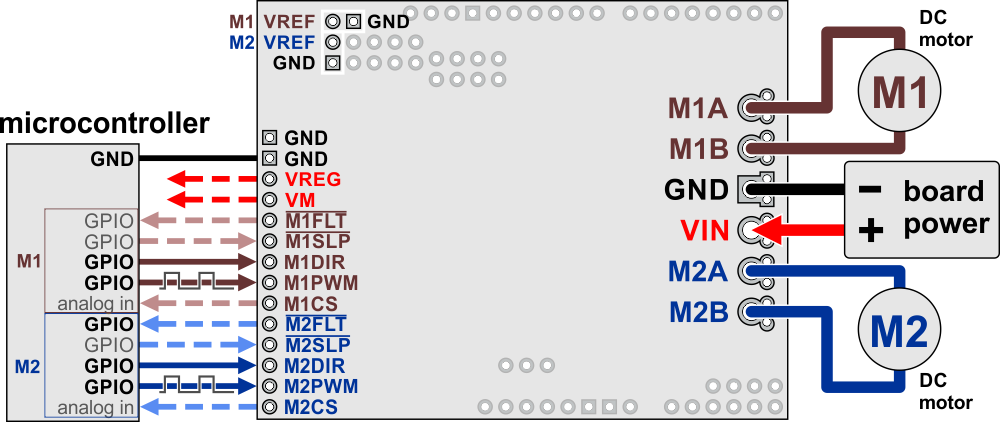
\includegraphics[scale=1.4]{images/pololu.png}
\caption{Schema delle connessioni del Pololu Dual G2.}
\end{figure}


\section{Microcontrollore}
La scheda di sviluppo scelta è una Nucleo STM32F767ZI.
Il processore è un Core Arm 32-bit Cortex-M7, ed è presente una Floating Point Unit per velocizzare le operazioni in virgola mobile.
La scheda ha 512kB di memoria RAM e 2MB di memoria FLASH.
È stata scelta per la grande disponibilità di periferiche integrate, in particolare per la realizzazione del sistema di controllo sono stati necessari: 
\begin{itemize}
    \item 2 timer a 32 bit per la gestione degli encoder.
    \item 1 timer a 16 bit per la generazione del segnale PWM.
    \item 1 periferica UART per la comunicazione con il computer.
\end{itemize}
Inoltre è presente un debugger integrato ST-LINK V2.1.

\begin{figure}[H]
\centering
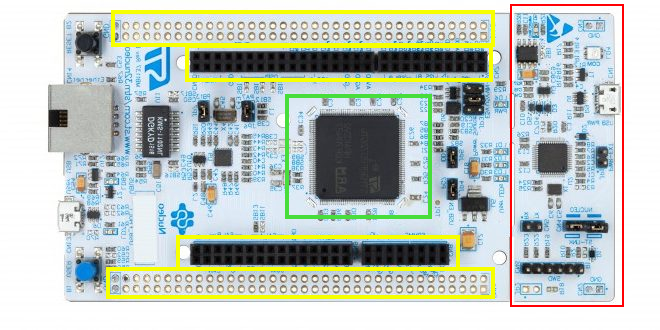
\includegraphics[scale=0.65]{images/nucleo.png}
\caption{La scheda Nucleo. Evidenziato in rosso il debugger, in verde il processore ed in giallo i GPIO per interfacciarsi con le varie periferiche.}
\end{figure}

\section{Modulo FTDI}
Per quanto riguarda la comunicazione tra microcontrollore e computer si è scelto il protocollo UART. 
Per rendere il sistema utilizzabile collegando un qualsiasi computer è stato necessario un modulo apposito che convertisse il segnale UART in un segnale USB, così da non dover utilizzare una piattaforma apposita dotata di GPIO. \\
È stato utilizzato un modulo FTDI FT232RL in quanto ampiamente supportato a livello di driver Linux e perché, oltre alle linee di trasmissione e ricezione, presenta alcuni meccanismi di controllo del flusso hardware tramite appositi pin (CTS e RTS) e un pin per poter effettuare il reset del microcontrollore direttamente dal PC.

\begin{figure}[H]
\centering
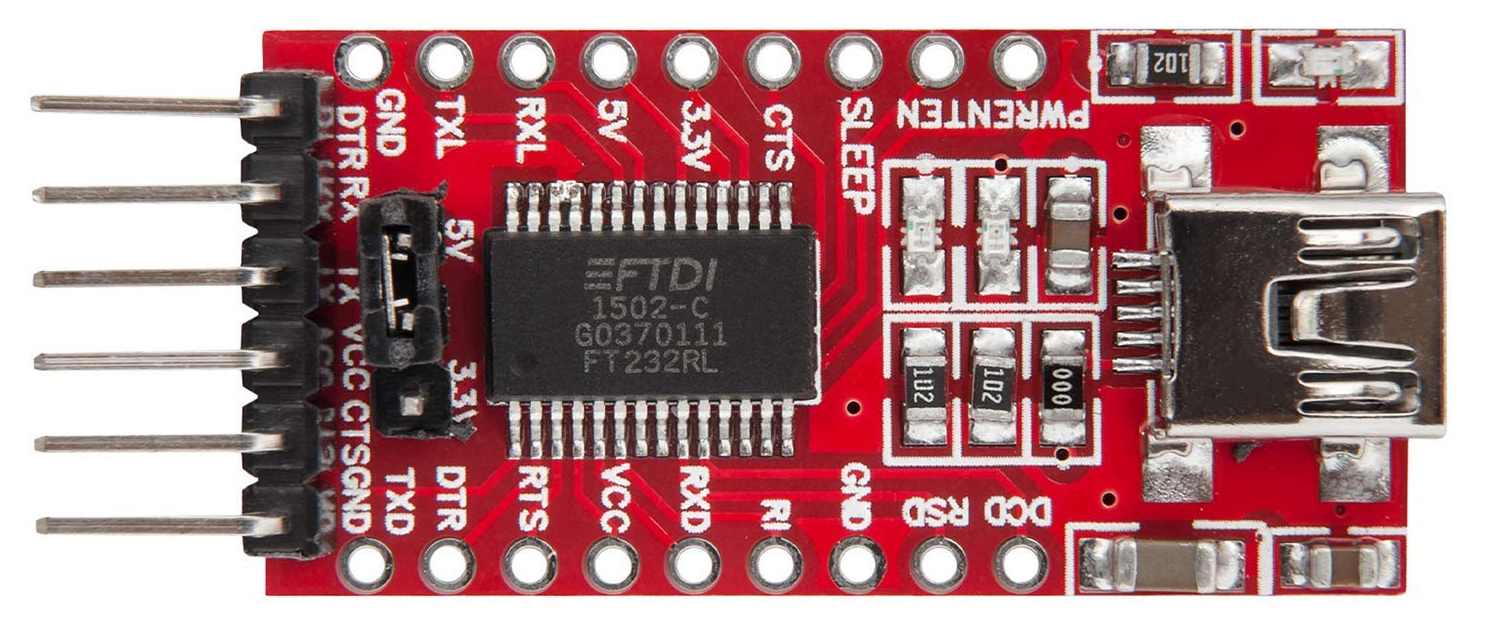
\includegraphics[scale=0.2]{images/ftdi.jpg}
\caption{Modulo FT232RL.}
\end{figure}
